\setlength{\columnsep}{3pt}
\begin{flushleft}

	\paragraph{What is DNS zone?}

	\begin{itemize}
		\item The DNS is broken up into many different zones. 
		\item \textbf{DNS zones encompass all records for a domain. }
		\item Eg: A zone for xzy.com would contain records such as www.xzy.com, support.xyz.com etc.
			\begin{figure}[h!]
			\centering
			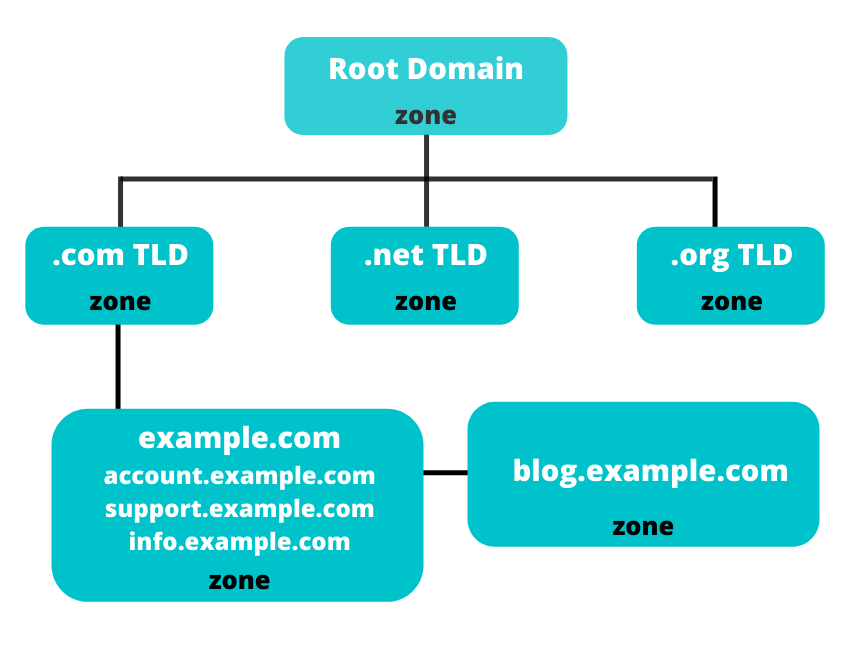
\includegraphics[scale=.55]{content/chapter3/images/zone.png}
			\caption{DNS zone}
			\label{fig:dns_heir32}
		\end{figure}
	\end{itemize}

	\paragraph{What is zone file?}
	\begin{itemize}
		\item A DNS zone file is a text file that maps domain names and IP addresses.
		\item They are human-readable and editable. 
		
	\end{itemize}
\end{flushleft}

\newpage





